\documentclass[1p]{elsarticle_modified}
%\bibliographystyle{elsarticle-num}

%\usepackage[colorlinks]{hyperref}
%\usepackage{abbrmath_seonhwa} %\Abb, \Ascr, \Acal ,\Abf, \Afrak
\usepackage{amsfonts}
\usepackage{amssymb}
\usepackage{amsmath}
\usepackage{amsthm}
\usepackage{scalefnt}
\usepackage{amsbsy}
\usepackage{kotex}
\usepackage{caption}
\usepackage{subfig}
\usepackage{color}
\usepackage{graphicx}
\usepackage{xcolor} %% white, black, red, green, blue, cyan, magenta, yellow
\usepackage{float}
\usepackage{setspace}
\usepackage{hyperref}

\usepackage{tikz}
\usetikzlibrary{arrows}

\usepackage{multirow}
\usepackage{array} % fixed length table
\usepackage{hhline}

%%%%%%%%%%%%%%%%%%%%%
\makeatletter
\renewcommand*\env@matrix[1][\arraystretch]{%
	\edef\arraystretch{#1}%
	\hskip -\arraycolsep
	\let\@ifnextchar\new@ifnextchar
	\array{*\c@MaxMatrixCols c}}
\makeatother %https://tex.stackexchange.com/questions/14071/how-can-i-increase-the-line-spacing-in-a-matrix
%%%%%%%%%%%%%%%

\usepackage[normalem]{ulem}

\newcommand{\msout}[1]{\ifmmode\text{\sout{\ensuremath{#1}}}\else\sout{#1}\fi}
%SOURCE: \msout is \stkout macro in https://tex.stackexchange.com/questions/20609/strikeout-in-math-mode

\newcommand{\cancel}[1]{
	\ifmmode
	{\color{red}\msout{#1}}
	\else
	{\color{red}\sout{#1}}
	\fi
}

\newcommand{\add}[1]{
	{\color{blue}\uwave{#1}}
}

\newcommand{\replace}[2]{
	\ifmmode
	{\color{red}\msout{#1}}{\color{blue}\uwave{#2}}
	\else
	{\color{red}\sout{#1}}{\color{blue}\uwave{#2}}
	\fi
}

\newcommand{\Sol}{\mathcal{S}} %segment
\newcommand{\D}{D} %diagram
\newcommand{\A}{\mathcal{A}} %arc


%%%%%%%%%%%%%%%%%%%%%%%%%%%%%5 test

\def\sl{\operatorname{\textup{SL}}(2,\Cbb)}
\def\psl{\operatorname{\textup{PSL}}(2,\Cbb)}
\def\quan{\mkern 1mu \triangleright \mkern 1mu}

\theoremstyle{definition}
\newtheorem{thm}{Theorem}[section]
\newtheorem{prop}[thm]{Proposition}
\newtheorem{lem}[thm]{Lemma}
\newtheorem{ques}[thm]{Question}
\newtheorem{cor}[thm]{Corollary}
\newtheorem{defn}[thm]{Definition}
\newtheorem{exam}[thm]{Example}
\newtheorem{rmk}[thm]{Remark}
\newtheorem{alg}[thm]{Algorithm}

\newcommand{\I}{\sqrt{-1}}
\begin{document}

%\begin{frontmatter}
%
%\title{Boundary parabolic representations of knots up to 8 crossings}
%
%%% Group authors per affiliation:
%\author{Yunhi Cho} 
%\address{Department of Mathematics, University of Seoul, Seoul, Korea}
%\ead{yhcho@uos.ac.kr}
%
%
%\author{Seonhwa Kim} %\fnref{s_kim}}
%\address{Center for Geometry and Physics, Institute for Basic Science, Pohang, 37673, Korea}
%\ead{ryeona17@ibs.re.kr}
%
%\author{Hyuk Kim}
%\address{Department of Mathematical Sciences, Seoul National University, Seoul 08826, Korea}
%\ead{hyukkim@snu.ac.kr}
%
%\author{Seokbeom Yoon}
%\address{Department of Mathematical Sciences, Seoul National University, Seoul, 08826,  Korea}
%\ead{sbyoon15@snu.ac.kr}
%
%\begin{abstract}
%We find all boundary parabolic representation of knots up to 8 crossings.
%
%\end{abstract}
%\begin{keyword}
%    \MSC[2010] 57M25 
%\end{keyword}
%
%\end{frontmatter}

%\linenumbers
%\tableofcontents
%
\newcommand\colored[1]{\textcolor{white}{\rule[-0.35ex]{0.8em}{1.4ex}}\kern-0.8em\color{red} #1}%
%\newcommand\colored[1]{\textcolor{white}{ #1}\kern-2.17ex	\textcolor{white}{ #1}\kern-1.81ex	\textcolor{white}{ #1}\kern-2.15ex\color{red}#1	}

{\Large $\underline{12n_{0318}~(K12n_{0318})}$}

\setlength{\tabcolsep}{10pt}
\renewcommand{\arraystretch}{1.6}
\vspace{1cm}\begin{tabular}{m{100pt}>{\centering\arraybackslash}m{274pt}}
\multirow{5}{120pt}{
	\centering
	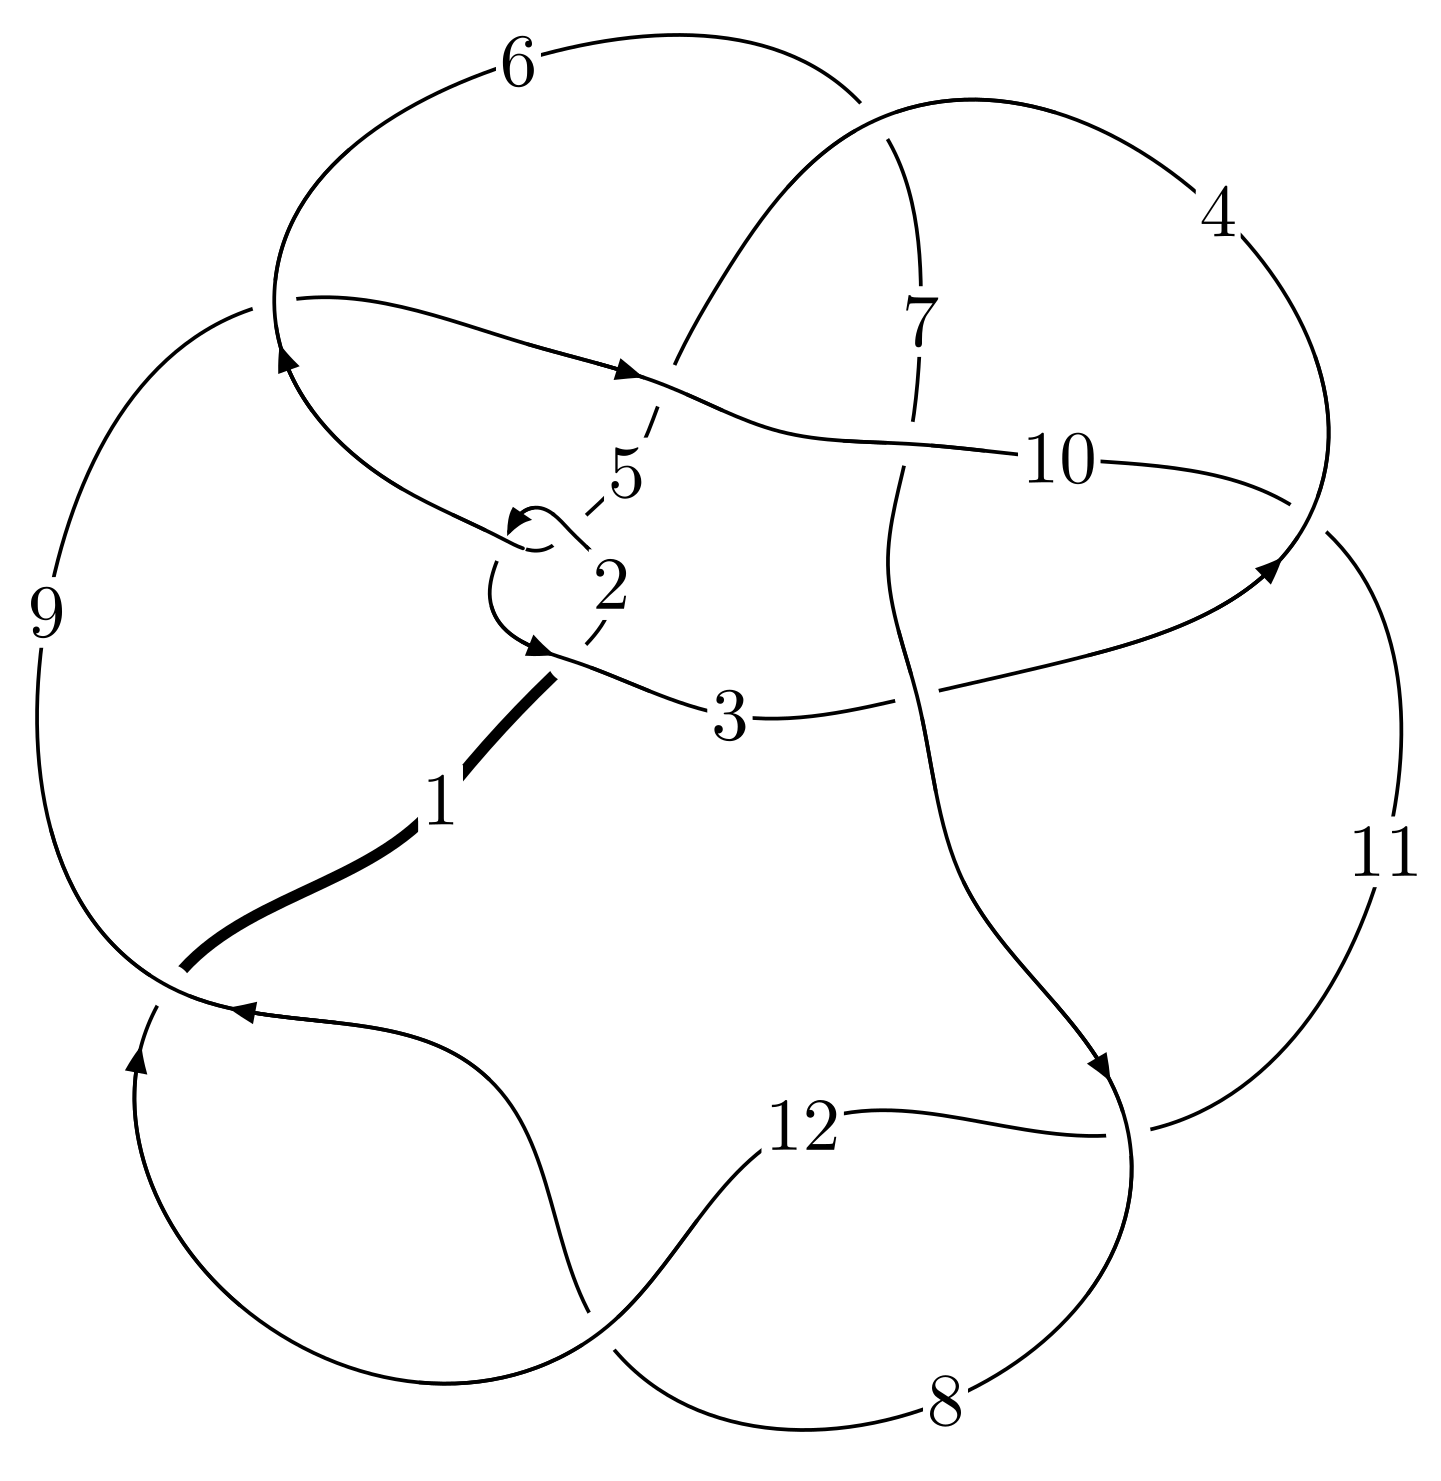
\includegraphics[width=112pt]{../../../GIT/diagram.site/Diagrams/png/2407_12n_0318.png}\\
\ \ \ A knot diagram\footnotemark}&
\allowdisplaybreaks
\textbf{Linearized knot diagam} \\
\cline{2-2}
 &
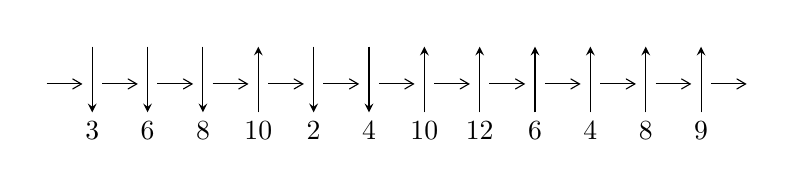
\begin{tikzpicture}[x=20pt, y=17pt]
	% nodes
	\node (C0) at (0, 0) {};
	\node (C1) at (1, 0) {};
	\node (C1U) at (1, +1) {};
	\node (C1D) at (1, -1) {3};

	\node (C2) at (2, 0) {};
	\node (C2U) at (2, +1) {};
	\node (C2D) at (2, -1) {6};

	\node (C3) at (3, 0) {};
	\node (C3U) at (3, +1) {};
	\node (C3D) at (3, -1) {8};

	\node (C4) at (4, 0) {};
	\node (C4U) at (4, +1) {};
	\node (C4D) at (4, -1) {10};

	\node (C5) at (5, 0) {};
	\node (C5U) at (5, +1) {};
	\node (C5D) at (5, -1) {2};

	\node (C6) at (6, 0) {};
	\node (C6U) at (6, +1) {};
	\node (C6D) at (6, -1) {4};

	\node (C7) at (7, 0) {};
	\node (C7U) at (7, +1) {};
	\node (C7D) at (7, -1) {10};

	\node (C8) at (8, 0) {};
	\node (C8U) at (8, +1) {};
	\node (C8D) at (8, -1) {12};

	\node (C9) at (9, 0) {};
	\node (C9U) at (9, +1) {};
	\node (C9D) at (9, -1) {6};

	\node (C10) at (10, 0) {};
	\node (C10U) at (10, +1) {};
	\node (C10D) at (10, -1) {4};

	\node (C11) at (11, 0) {};
	\node (C11U) at (11, +1) {};
	\node (C11D) at (11, -1) {8};

	\node (C12) at (12, 0) {};
	\node (C12U) at (12, +1) {};
	\node (C12D) at (12, -1) {9};
	\node (C13) at (13, 0) {};

	% arrows
	\draw[->,>={angle 60}]
	(C0) edge (C1) (C1) edge (C2) (C2) edge (C3) (C3) edge (C4) (C4) edge (C5) (C5) edge (C6) (C6) edge (C7) (C7) edge (C8) (C8) edge (C9) (C9) edge (C10) (C10) edge (C11) (C11) edge (C12) (C12) edge (C13) ;	\draw[->,>=stealth]
	(C1U) edge (C1D) (C2U) edge (C2D) (C3U) edge (C3D) (C4D) edge (C4U) (C5U) edge (C5D) (C6U) edge (C6D) (C7D) edge (C7U) (C8D) edge (C8U) (C9D) edge (C9U) (C10D) edge (C10U) (C11D) edge (C11U) (C12D) edge (C12U) ;
	\end{tikzpicture} \\
\hhline{~~} \\& 
\textbf{Solving Sequence} \\ \cline{2-2} 
 &
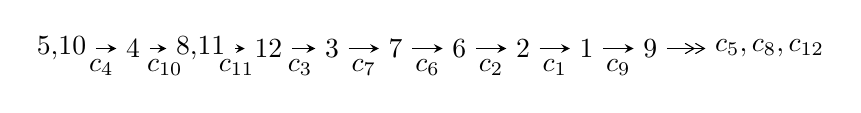
\begin{tikzpicture}[x=23pt, y=7pt]
	% node
	\node (A0) at (-1/8, 0) {5,10};
	\node (A1) at (1, 0) {4};
	\node (A2) at (33/16, 0) {8,11};
	\node (A3) at (25/8, 0) {12};
	\node (A4) at (33/8, 0) {3};
	\node (A5) at (41/8, 0) {7};
	\node (A6) at (49/8, 0) {6};
	\node (A7) at (57/8, 0) {2};
	\node (A8) at (65/8, 0) {1};
	\node (A9) at (73/8, 0) {9};
	\node (C1) at (1/2, -1) {$c_{4}$};
	\node (C2) at (3/2, -1) {$c_{10}$};
	\node (C3) at (21/8, -1) {$c_{11}$};
	\node (C4) at (29/8, -1) {$c_{3}$};
	\node (C5) at (37/8, -1) {$c_{7}$};
	\node (C6) at (45/8, -1) {$c_{6}$};
	\node (C7) at (53/8, -1) {$c_{2}$};
	\node (C8) at (61/8, -1) {$c_{1}$};
	\node (C9) at (69/8, -1) {$c_{9}$};
	\node (A10) at (11, 0) {$c_{5},c_{8},c_{12}$};

	% edge
	\draw[->,>=stealth]	
	(A0) edge (A1) (A1) edge (A2) (A2) edge (A3) (A3) edge (A4) (A4) edge (A5) (A5) edge (A6) (A6) edge (A7) (A7) edge (A8) (A8) edge (A9) ;
	\draw[->>,>={angle 60}]	
	(A9) edge (A10);
\end{tikzpicture} \\ 

\end{tabular} \\

\footnotetext{
The image of knot diagram is generated by the software ``\textbf{Draw programme}" developed by Andrew Bartholomew(\url{http://www.layer8.co.uk/maths/draw/index.htm\#Running-draw}), where we modified some parts for our purpose(\url{https://github.com/CATsTAILs/LinksPainter}).
}\phantom \\ \newline 
\centering \textbf{Ideals for irreducible components\footnotemark of $X_{\text{par}}$} 
 
\begin{align*}
I^u_{1}&=\langle 
-46 u^9+96 u^8-471 u^7+631 u^6-1426 u^5+1075 u^4-1285 u^3+249 u^2+61 b-157 u-203,\\
\phantom{I^u_{1}}&\phantom{= \langle  }-3 u^9+5 u^8-28 u^7+29 u^6-74 u^5+37 u^4-51 u^3+u^2+a-5 u-8,\\
\phantom{I^u_{1}}&\phantom{= \langle  }u^{10}-2 u^9+10 u^8-13 u^7+29 u^6-22 u^5+24 u^4-8 u^3+3 u^2+2 u-1\rangle \\
I^u_{2}&=\langle 
4 u^9-38 u^8+23 u^7-323 u^6+100 u^5-821 u^4+395 u^3-595 u^2+185 b+617 u-243,\\
\phantom{I^u_{2}}&\phantom{= \langle  }-439 u^9-177 u^8-3588 u^7-117 u^6-9310 u^5+2461 u^4-8895 u^3+5315 u^2+185 a-3937 u+1278,\\
\phantom{I^u_{2}}&\phantom{= \langle  }u^{10}+8 u^8-3 u^7+21 u^6-14 u^5+22 u^4-20 u^3+13 u^2-6 u+1\rangle \\
\\
\end{align*}
\raggedright * 2 irreducible components of $\dim_{\mathbb{C}}=0$, with total 20 representations.\\
\footnotetext{All coefficients of polynomials are rational numbers. But the coefficients are sometimes approximated in decimal forms when there is not enough margin.}
\newpage
\renewcommand{\arraystretch}{1}
\centering \section*{I. $I^u_{1}= \langle -46 u^9+96 u^8+\cdots+61 b-203,\;-3 u^9+5 u^8+\cdots+a-8,\;u^{10}-2 u^9+\cdots+2 u-1 \rangle$}
\flushleft \textbf{(i) Arc colorings}\\
\begin{tabular}{m{7pt} m{180pt} m{7pt} m{180pt} }
\flushright $a_{5}=$&$\begin{pmatrix}1\\0\end{pmatrix}$ \\
\flushright $a_{10}=$&$\begin{pmatrix}0\\u\end{pmatrix}$ \\
\flushright $a_{4}=$&$\begin{pmatrix}1\\u^2\end{pmatrix}$ \\
\flushright $a_{8}=$&$\begin{pmatrix}3 u^9-5 u^8+28 u^7-29 u^6+74 u^5-37 u^4+51 u^3- u^2+5 u+8\\0.754098 u^{9}-1.57377 u^{8}+\cdots+2.57377 u+3.32787\end{pmatrix}$ \\
\flushright $a_{11}=$&$\begin{pmatrix}u\\u^3+u\end{pmatrix}$ \\
\flushright $a_{12}=$&$\begin{pmatrix}7.27869 u^{9}-12.0164 u^{8}+\cdots+22.0164 u+22.2951\\3.27869 u^{9}-5.01639 u^{8}+\cdots+9.01639 u+8.29508\end{pmatrix}$ \\
\flushright $a_{3}=$&$\begin{pmatrix}-7.70492 u^{9}+12.6885 u^{8}+\cdots-21.6885 u-22.3934\\-3.40984 u^{9}+5.37705 u^{8}+\cdots-8.37705 u-8.78689\end{pmatrix}$ \\
\flushright $a_{7}=$&$\begin{pmatrix}3 u^9-5 u^8+28 u^7-29 u^6+74 u^5-37 u^4+51 u^3- u^2+5 u+8\\0.754098 u^{9}-1.57377 u^{8}+\cdots+3.57377 u+4.32787\end{pmatrix}$ \\
\flushright $a_{6}=$&$\begin{pmatrix}3.75410 u^{9}-6.57377 u^{8}+\cdots+7.57377 u+11.3279\\0.803279 u^{9}-1.45902 u^{8}+\cdots+4.45902 u+4.26230\end{pmatrix}$ \\
\flushright $a_{2}=$&$\begin{pmatrix}1.26230 u^{9}-1.72131 u^{8}+\cdots+2.72131 u+3.98361\\0.983607 u^{9}-1.70492 u^{8}+\cdots+0.704918 u+1.68852\end{pmatrix}$ \\
\flushright $a_{1}=$&$\begin{pmatrix}51.8033 u^{9}-86.4590 u^{8}+\cdots+129.459 u+150.262\\19.7377 u^{9}-31.2787 u^{8}+\cdots+54.2787 u+58.0164\end{pmatrix}$ \\
\flushright $a_{9}=$&$\begin{pmatrix}-20.5410 u^{9}+33.7377 u^{8}+\cdots-52.7377 u-58.2787\\-8.31148 u^{9}+14.6066 u^{8}+\cdots-18.6066 u-23.9180\end{pmatrix}$\\&\end{tabular}
\flushleft \textbf{(ii) Obstruction class $= -1$}\\~\\
\flushleft \textbf{(iii) Cusp Shapes $= -\frac{62}{61} u^9+\frac{201}{61} u^8-\frac{725}{61} u^7+\frac{1487}{61} u^6-\frac{2349}{61} u^5+\frac{3080}{61} u^4-\frac{2090}{61} u^3+\frac{1667}{61} u^2-\frac{445}{61} u+\frac{103}{61}$}\\~\\
\newpage\renewcommand{\arraystretch}{1}
\flushleft \textbf{(iv) u-Polynomials at the component}\newline \\
\begin{tabular}{m{50pt}|m{274pt}}
Crossings & \hspace{64pt}u-Polynomials at each crossing \\
\hline $$\begin{aligned}c_{1}\end{aligned}$$&$\begin{aligned}
&u^{10}+22 u^9+\cdots+5917 u+49
\end{aligned}$\\
\hline $$\begin{aligned}c_{2},c_{5}\end{aligned}$$&$\begin{aligned}
&u^{10}+2 u^9+\cdots-59 u+7
\end{aligned}$\\
\hline $$\begin{aligned}c_{3}\end{aligned}$$&$\begin{aligned}
&u^{10}+3 u^9+\cdots+12 u-13
\end{aligned}$\\
\hline $$\begin{aligned}c_{4},c_{10}\end{aligned}$$&$\begin{aligned}
&u^{10}+2 u^9+10 u^8+13 u^7+29 u^6+22 u^5+24 u^4+8 u^3+3 u^2-2 u-1
\end{aligned}$\\
\hline $$\begin{aligned}c_{6}\end{aligned}$$&$\begin{aligned}
&u^{10}-3 u^9+\cdots+110 u-25
\end{aligned}$\\
\hline $$\begin{aligned}c_{7}\end{aligned}$$&$\begin{aligned}
&u^{10}+3 u^9-20 u^7-41 u^6+294 u^5-405 u^4+219 u^3+58 u^2-33 u-9
\end{aligned}$\\
\hline $$\begin{aligned}c_{8},c_{11},c_{12}\end{aligned}$$&$\begin{aligned}
&u^{10}-3 u^9+\cdots+37 u-29
\end{aligned}$\\
\hline $$\begin{aligned}c_{9}\end{aligned}$$&$\begin{aligned}
&u^{10}+u^9+\cdots-25 u-167
\end{aligned}$\\
\hline
\end{tabular}\\~\\
\newpage\renewcommand{\arraystretch}{1}
\flushleft \textbf{(v) Riley Polynomials at the component}\newline \\
\begin{tabular}{m{50pt}|m{274pt}}
Crossings & \hspace{64pt}Riley Polynomials at each crossing \\
\hline $$\begin{aligned}c_{1}\end{aligned}$$&$\begin{aligned}
&y^{10}-34 y^9+\cdots-33340185 y+2401
\end{aligned}$\\
\hline $$\begin{aligned}c_{2},c_{5}\end{aligned}$$&$\begin{aligned}
&y^{10}-22 y^9+\cdots-5917 y+49
\end{aligned}$\\
\hline $$\begin{aligned}c_{3}\end{aligned}$$&$\begin{aligned}
&y^{10}-19 y^9+\cdots-2666 y+169
\end{aligned}$\\
\hline $$\begin{aligned}c_{4},c_{10}\end{aligned}$$&$\begin{aligned}
&y^{10}+16 y^9+\cdots-10 y+1
\end{aligned}$\\
\hline $$\begin{aligned}c_{6}\end{aligned}$$&$\begin{aligned}
&y^{10}-27 y^9+\cdots-23900 y+625
\end{aligned}$\\
\hline $$\begin{aligned}c_{7}\end{aligned}$$&$\begin{aligned}
&y^{10}-9 y^9+\cdots-2133 y+81
\end{aligned}$\\
\hline $$\begin{aligned}c_{8},c_{11},c_{12}\end{aligned}$$&$\begin{aligned}
&y^{10}-21 y^9+\cdots+3097 y+841
\end{aligned}$\\
\hline $$\begin{aligned}c_{9}\end{aligned}$$&$\begin{aligned}
&y^{10}-17 y^9+\cdots-55401 y+27889
\end{aligned}$\\
\hline
\end{tabular}\\~\\
\newpage\flushleft \textbf{(vi) Complex Volumes and Cusp Shapes}
$$\begin{array}{c|c|c}  
\text{Solutions to }I^u_{1}& \I (\text{vol} + \sqrt{-1}CS) & \text{Cusp shape}\\
 \hline 
\begin{aligned}
u &= \phantom{-}0.058067 + 0.959343 I \\
a &= -1.02272 + 1.68359 I \\
b &= -0.56593 - 1.71994 I\end{aligned}
 & \phantom{-}2.74627 + 1.52551 I & \phantom{-}1.61031 - 1.19705 I \\ \hline\begin{aligned}
u &= \phantom{-}0.058067 - 0.959343 I \\
a &= -1.02272 - 1.68359 I \\
b &= -0.56593 + 1.71994 I\end{aligned}
 & \phantom{-}2.74627 - 1.52551 I & \phantom{-}1.61031 + 1.19705 I \\ \hline\begin{aligned}
u &= \phantom{-}0.369407 + 0.683035 I \\
a &= \phantom{-}0.045927 - 0.332128 I \\
b &= \phantom{-}0.679565 + 0.238520 I\end{aligned}
 & -1.42142 - 0.67316 I & -3.66351 + 1.21479 I \\ \hline\begin{aligned}
u &= \phantom{-}0.369407 - 0.683035 I \\
a &= \phantom{-}0.045927 + 0.332128 I \\
b &= \phantom{-}0.679565 - 0.238520 I\end{aligned}
 & -1.42142 + 0.67316 I & -3.66351 - 1.21479 I \\ \hline\begin{aligned}
u &= -0.387852\phantom{ +0.000000I} \\
a &= \phantom{-}1.30915\phantom{ +0.000000I} \\
b &= -0.163807\phantom{ +0.000000I}\end{aligned}
 & \phantom{-}0.892115\phantom{ +0.000000I} & \phantom{-}12.2090\phantom{ +0.000000I} \\ \hline\begin{aligned}
u &= \phantom{-}0.346316\phantom{ +0.000000I} \\
a &= \phantom{-}11.5322\phantom{ +0.000000I} \\
b &= \phantom{-}4.45406\phantom{ +0.000000I}\end{aligned}
 & \phantom{-}5.57991\phantom{ +0.000000I} & \phantom{-}1.58660\phantom{ +0.000000I} \\ \hline\begin{aligned}
u &= \phantom{-}0.45233 + 1.77782 I \\
a &= -0.557671 + 0.304853 I \\
b &= -0.225028 - 1.028840 I\end{aligned}
 & -9.90958 + 3.92064 I & \phantom{-}1.45511 - 3.03765 I \\ \hline\begin{aligned}
u &= \phantom{-}0.45233 - 1.77782 I \\
a &= -0.557671 - 0.304853 I \\
b &= -0.225028 + 1.028840 I\end{aligned}
 & -9.90958 - 3.92064 I & \phantom{-}1.45511 + 3.03765 I \\ \hline\begin{aligned}
u &= \phantom{-}0.14096 + 1.98796 I \\
a &= \phantom{-}1.61376 - 0.88253 I \\
b &= -3.53373 + 2.38309 I\end{aligned}
 & \phantom{-}15.2183 + 8.0662 I & \phantom{-}1.70029 - 2.38226 I \\ \hline\begin{aligned}
u &= \phantom{-}0.14096 - 1.98796 I \\
a &= \phantom{-}1.61376 + 0.88253 I \\
b &= -3.53373 - 2.38309 I\end{aligned}
 & \phantom{-}15.2183 - 8.0662 I & \phantom{-}1.70029 + 2.38226 I\\
 \hline 
 \end{array}$$\newpage\newpage\renewcommand{\arraystretch}{1}
\centering \section*{II. $I^u_{2}= \langle 4 u^9-38 u^8+\cdots+185 b-243,\;-439 u^9-177 u^8+\cdots+185 a+1278,\;u^{10}+8 u^8+\cdots-6 u+1 \rangle$}
\flushleft \textbf{(i) Arc colorings}\\
\begin{tabular}{m{7pt} m{180pt} m{7pt} m{180pt} }
\flushright $a_{5}=$&$\begin{pmatrix}1\\0\end{pmatrix}$ \\
\flushright $a_{10}=$&$\begin{pmatrix}0\\u\end{pmatrix}$ \\
\flushright $a_{4}=$&$\begin{pmatrix}1\\u^2\end{pmatrix}$ \\
\flushright $a_{8}=$&$\begin{pmatrix}2.37297 u^{9}+0.956757 u^{8}+\cdots+21.2811 u-6.90811\\-0.0216216 u^{9}+0.205405 u^{8}+\cdots-3.33514 u+1.31351\end{pmatrix}$ \\
\flushright $a_{11}=$&$\begin{pmatrix}u\\u^3+u\end{pmatrix}$ \\
\flushright $a_{12}=$&$\begin{pmatrix}1.37297 u^{9}+0.956757 u^{8}+\cdots+9.28108 u-0.908108\\0.432432 u^{9}-0.108108 u^{8}+\cdots+8.70270 u-2.27027\end{pmatrix}$ \\
\flushright $a_{3}=$&$\begin{pmatrix}-0.745946 u^{9}+0.0864865 u^{8}+\cdots-7.56216 u+3.81622\\0.745946 u^{9}-0.0864865 u^{8}+\cdots+7.56216 u-1.81622\end{pmatrix}$ \\
\flushright $a_{7}=$&$\begin{pmatrix}2.37297 u^{9}+0.956757 u^{8}+\cdots+21.2811 u-6.90811\\0.389189 u^{9}+0.302703 u^{8}+\cdots+0.0324324 u+0.356757\end{pmatrix}$ \\
\flushright $a_{6}=$&$\begin{pmatrix}2.35135 u^{9}+1.16216 u^{8}+\cdots+17.9459 u-5.59459\\0.437838 u^{9}+0.340541 u^{8}+\cdots+1.28649 u+0.151351\end{pmatrix}$ \\
\flushright $a_{2}=$&$\begin{pmatrix}-3.11892 u^{9}-0.870270 u^{8}+\cdots-28.8432 u+9.72432\\0.313514 u^{9}+0.0216216 u^{8}+\cdots+0.859459 u-0.545946\end{pmatrix}$ \\
\flushright $a_{1}=$&$\begin{pmatrix}-3.24324 u^{9}-1.18919 u^{8}+\cdots-29.2703 u+9.02703\\-0.702703 u^{9}-0.324324 u^{8}+\cdots-2.89189 u+0.189189\end{pmatrix}$ \\
\flushright $a_{9}=$&$\begin{pmatrix}-2.24324 u^{9}-1.18919 u^{8}+\cdots-17.2703 u+4.02703\\-1.14054 u^{9}-0.664865 u^{8}+\cdots-6.17838 u+2.03784\end{pmatrix}$\\&\end{tabular}
\flushleft \textbf{(ii) Obstruction class $= 1$}\\~\\
\flushleft \textbf{(iii) Cusp Shapes $= \frac{1244}{185} u^9+\frac{577}{185} u^8+\frac{10113}{185} u^7+\frac{927}{185} u^6+\frac{5147}{37} u^5-\frac{5396}{185} u^4+\frac{4552}{37} u^3-\frac{2673}{37} u^2+\frac{7997}{185} u-\frac{1943}{185}$}\\~\\
\newpage\renewcommand{\arraystretch}{1}
\flushleft \textbf{(iv) u-Polynomials at the component}\newline \\
\begin{tabular}{m{50pt}|m{274pt}}
Crossings & \hspace{64pt}u-Polynomials at each crossing \\
\hline $$\begin{aligned}c_{1}\end{aligned}$$&$\begin{aligned}
&u^{10}-10 u^9+\cdots-13 u+1
\end{aligned}$\\
\hline $$\begin{aligned}c_{2}\end{aligned}$$&$\begin{aligned}
&u^{10}+2 u^9-3 u^8-7 u^7+4 u^6+12 u^5- u^4-11 u^3-2 u^2+3 u+1
\end{aligned}$\\
\hline $$\begin{aligned}c_{3}\end{aligned}$$&$\begin{aligned}
&u^{10}+u^9- u^8- u^6-3 u^5+3 u^4- u^3+5 u^2-2 u-1
\end{aligned}$\\
\hline $$\begin{aligned}c_{4}\end{aligned}$$&$\begin{aligned}
&u^{10}+8 u^8-3 u^7+21 u^6-14 u^5+22 u^4-20 u^3+13 u^2-6 u+1
\end{aligned}$\\
\hline $$\begin{aligned}c_{5}\end{aligned}$$&$\begin{aligned}
&u^{10}-2 u^9-3 u^8+7 u^7+4 u^6-12 u^5- u^4+11 u^3-2 u^2-3 u+1
\end{aligned}$\\
\hline $$\begin{aligned}c_{6}\end{aligned}$$&$\begin{aligned}
&u^{10}+3 u^9+u^8-4 u^7-8 u^6-9 u^5+11 u^4+31 u^3+24 u^2+8 u+1
\end{aligned}$\\
\hline $$\begin{aligned}c_{7}\end{aligned}$$&$\begin{aligned}
&u^{10}+u^9+4 u^8+4 u^7-3 u^6-8 u^5-13 u^4-21 u^3-18 u^2-7 u-1
\end{aligned}$\\
\hline $$\begin{aligned}c_{8}\end{aligned}$$&$\begin{aligned}
&u^{10}-3 u^9+9 u^7-8 u^6-7 u^5+11 u^4- u^3-3 u^2+u-1
\end{aligned}$\\
\hline $$\begin{aligned}c_{9}\end{aligned}$$&$\begin{aligned}
&u^{10}- u^9+2 u^8+u^7-11 u^6+10 u^5-7 u^4+2 u^3+4 u^2+u-1
\end{aligned}$\\
\hline $$\begin{aligned}c_{10}\end{aligned}$$&$\begin{aligned}
&u^{10}+8 u^8+3 u^7+21 u^6+14 u^5+22 u^4+20 u^3+13 u^2+6 u+1
\end{aligned}$\\
\hline $$\begin{aligned}c_{11},c_{12}\end{aligned}$$&$\begin{aligned}
&u^{10}+3 u^9-9 u^7-8 u^6+7 u^5+11 u^4+u^3-3 u^2- u-1
\end{aligned}$\\
\hline
\end{tabular}\\~\\
\newpage\renewcommand{\arraystretch}{1}
\flushleft \textbf{(v) Riley Polynomials at the component}\newline \\
\begin{tabular}{m{50pt}|m{274pt}}
Crossings & \hspace{64pt}Riley Polynomials at each crossing \\
\hline $$\begin{aligned}c_{1}\end{aligned}$$&$\begin{aligned}
&y^{10}-10 y^9+\cdots-33 y+1
\end{aligned}$\\
\hline $$\begin{aligned}c_{2},c_{5}\end{aligned}$$&$\begin{aligned}
&y^{10}-10 y^9+\cdots-13 y+1
\end{aligned}$\\
\hline $$\begin{aligned}c_{3}\end{aligned}$$&$\begin{aligned}
&y^{10}-3 y^9- y^8+14 y^7+7 y^6-23 y^5-5 y^4+19 y^3+15 y^2-14 y+1
\end{aligned}$\\
\hline $$\begin{aligned}c_{4},c_{10}\end{aligned}$$&$\begin{aligned}
&y^{10}+16 y^9+\cdots-10 y+1
\end{aligned}$\\
\hline $$\begin{aligned}c_{6}\end{aligned}$$&$\begin{aligned}
&y^{10}-7 y^9+\cdots-16 y+1
\end{aligned}$\\
\hline $$\begin{aligned}c_{7}\end{aligned}$$&$\begin{aligned}
&y^{10}+7 y^9+\cdots-13 y+1
\end{aligned}$\\
\hline $$\begin{aligned}c_{8},c_{11},c_{12}\end{aligned}$$&$\begin{aligned}
&y^{10}-9 y^9+\cdots+5 y+1
\end{aligned}$\\
\hline $$\begin{aligned}c_{9}\end{aligned}$$&$\begin{aligned}
&y^{10}+3 y^9+\cdots-9 y+1
\end{aligned}$\\
\hline
\end{tabular}\\~\\
\newpage\flushleft \textbf{(vi) Complex Volumes and Cusp Shapes}
$$\begin{array}{c|c|c}  
\text{Solutions to }I^u_{2}& \I (\text{vol} + \sqrt{-1}CS) & \text{Cusp shape}\\
 \hline 
\begin{aligned}
u &= -0.421587 + 1.150120 I \\
a &= -0.068626 + 0.779782 I \\
b &= \phantom{-}0.442051 + 0.121008 I\end{aligned}
 & -0.46461 + 1.98898 I & -0.06537 - 3.20823 I \\ \hline\begin{aligned}
u &= -0.421587 - 1.150120 I \\
a &= -0.068626 - 0.779782 I \\
b &= \phantom{-}0.442051 - 0.121008 I\end{aligned}
 & -0.46461 - 1.98898 I & -0.06537 + 3.20823 I \\ \hline\begin{aligned}
u &= \phantom{-}0.235261 + 0.587721 I \\
a &= -0.300901 + 0.648896 I \\
b &= \phantom{-}0.14149 - 1.45935 I\end{aligned}
 & \phantom{-}5.08555 + 2.55932 I & \phantom{-}4.45408 - 5.37582 I \\ \hline\begin{aligned}
u &= \phantom{-}0.235261 - 0.587721 I \\
a &= -0.300901 - 0.648896 I \\
b &= \phantom{-}0.14149 + 1.45935 I\end{aligned}
 & \phantom{-}5.08555 - 2.55932 I & \phantom{-}4.45408 + 5.37582 I \\ \hline\begin{aligned}
u &= \phantom{-}0.490498\phantom{ +0.000000I} \\
a &= \phantom{-}3.09930\phantom{ +0.000000I} \\
b &= \phantom{-}0.465102\phantom{ +0.000000I}\end{aligned}
 & \phantom{-}6.94382\phantom{ +0.000000I} & \phantom{-}10.5630\phantom{ +0.000000I} \\ \hline\begin{aligned}
u &= \phantom{-}0.12366 + 1.64371 I \\
a &= -1.257140 - 0.128400 I \\
b &= \phantom{-}1.83592 + 0.29637 I\end{aligned}
 & -6.58180 + 1.84846 I & \phantom{-}1.62067 - 1.24709 I \\ \hline\begin{aligned}
u &= \phantom{-}0.12366 - 1.64371 I \\
a &= -1.257140 + 0.128400 I \\
b &= \phantom{-}1.83592 - 0.29637 I\end{aligned}
 & -6.58180 - 1.84846 I & \phantom{-}1.62067 + 1.24709 I \\ \hline\begin{aligned}
u &= \phantom{-}0.293026\phantom{ +0.000000I} \\
a &= -1.91458\phantom{ +0.000000I} \\
b &= \phantom{-}0.591313\phantom{ +0.000000I}\end{aligned}
 & \phantom{-}0.102739\phantom{ +0.000000I} & -0.844670\phantom{ +0.000000I} \\ \hline\begin{aligned}
u &= -0.32909 + 2.03714 I \\
a &= \phantom{-}0.534307 - 0.226160 I \\
b &= -1.44767 + 0.48227 I\end{aligned}
 & -11.43200 - 3.15494 I & -2.86863 + 1.76027 I \\ \hline\begin{aligned}
u &= -0.32909 - 2.03714 I \\
a &= \phantom{-}0.534307 + 0.226160 I \\
b &= -1.44767 - 0.48227 I\end{aligned}
 & -11.43200 + 3.15494 I & -2.86863 - 1.76027 I\\
 \hline 
 \end{array}$$\newpage
\newpage\renewcommand{\arraystretch}{1}
\centering \section*{ III. u-Polynomials}
\begin{tabular}{m{50pt}|m{274pt}}
Crossings & \hspace{64pt}u-Polynomials at each crossing \\
\hline $$\begin{aligned}c_{1}\end{aligned}$$&$\begin{aligned}
&(u^{10}-10 u^9+\cdots-13 u+1)(u^{10}+22 u^9+\cdots+5917 u+49)
\end{aligned}$\\
\hline $$\begin{aligned}c_{2}\end{aligned}$$&$\begin{aligned}
&(u^{10}+2 u^9+\cdots-59 u+7)\\
&\cdot(u^{10}+2 u^9-3 u^8-7 u^7+4 u^6+12 u^5- u^4-11 u^3-2 u^2+3 u+1)
\end{aligned}$\\
\hline $$\begin{aligned}c_{3}\end{aligned}$$&$\begin{aligned}
&(u^{10}+u^9- u^8- u^6-3 u^5+3 u^4- u^3+5 u^2-2 u-1)\\
&\cdot(u^{10}+3 u^9+\cdots+12 u-13)
\end{aligned}$\\
\hline $$\begin{aligned}c_{4}\end{aligned}$$&$\begin{aligned}
&(u^{10}+8 u^8-3 u^7+21 u^6-14 u^5+22 u^4-20 u^3+13 u^2-6 u+1)\\
&\cdot(u^{10}+2 u^9+10 u^8+13 u^7+29 u^6+22 u^5+24 u^4+8 u^3+3 u^2-2 u-1)
\end{aligned}$\\
\hline $$\begin{aligned}c_{5}\end{aligned}$$&$\begin{aligned}
&(u^{10}-2 u^9-3 u^8+7 u^7+4 u^6-12 u^5- u^4+11 u^3-2 u^2-3 u+1)\\
&\cdot(u^{10}+2 u^9+\cdots-59 u+7)
\end{aligned}$\\
\hline $$\begin{aligned}c_{6}\end{aligned}$$&$\begin{aligned}
&(u^{10}-3 u^9+\cdots+110 u-25)\\
&\cdot(u^{10}+3 u^9+u^8-4 u^7-8 u^6-9 u^5+11 u^4+31 u^3+24 u^2+8 u+1)
\end{aligned}$\\
\hline $$\begin{aligned}c_{7}\end{aligned}$$&$\begin{aligned}
&(u^{10}+u^9+4 u^8+4 u^7-3 u^6-8 u^5-13 u^4-21 u^3-18 u^2-7 u-1)\\
&\cdot(u^{10}+3 u^9-20 u^7-41 u^6+294 u^5-405 u^4+219 u^3+58 u^2-33 u-9)
\end{aligned}$\\
\hline $$\begin{aligned}c_{8}\end{aligned}$$&$\begin{aligned}
&(u^{10}-3 u^9+9 u^7-8 u^6-7 u^5+11 u^4- u^3-3 u^2+u-1)\\
&\cdot(u^{10}-3 u^9+\cdots+37 u-29)
\end{aligned}$\\
\hline $$\begin{aligned}c_{9}\end{aligned}$$&$\begin{aligned}
&(u^{10}- u^9+2 u^8+u^7-11 u^6+10 u^5-7 u^4+2 u^3+4 u^2+u-1)\\
&\cdot(u^{10}+u^9+\cdots-25 u-167)
\end{aligned}$\\
\hline $$\begin{aligned}c_{10}\end{aligned}$$&$\begin{aligned}
&(u^{10}+8 u^8+3 u^7+21 u^6+14 u^5+22 u^4+20 u^3+13 u^2+6 u+1)\\
&\cdot(u^{10}+2 u^9+10 u^8+13 u^7+29 u^6+22 u^5+24 u^4+8 u^3+3 u^2-2 u-1)
\end{aligned}$\\
\hline $$\begin{aligned}c_{11},c_{12}\end{aligned}$$&$\begin{aligned}
&(u^{10}-3 u^9+\cdots+37 u-29)\\
&\cdot(u^{10}+3 u^9-9 u^7-8 u^6+7 u^5+11 u^4+u^3-3 u^2- u-1)
\end{aligned}$\\
\hline
\end{tabular}\newpage\renewcommand{\arraystretch}{1}
\centering \section*{ IV. Riley Polynomials}
\begin{tabular}{m{50pt}|m{274pt}}
Crossings & \hspace{64pt}Riley Polynomials at each crossing \\
\hline $$\begin{aligned}c_{1}\end{aligned}$$&$\begin{aligned}
&(y^{10}-34 y^9+\cdots-33340185 y+2401)(y^{10}-10 y^9+\cdots-33 y+1)
\end{aligned}$\\
\hline $$\begin{aligned}c_{2},c_{5}\end{aligned}$$&$\begin{aligned}
&(y^{10}-22 y^9+\cdots-5917 y+49)(y^{10}-10 y^9+\cdots-13 y+1)
\end{aligned}$\\
\hline $$\begin{aligned}c_{3}\end{aligned}$$&$\begin{aligned}
&(y^{10}-19 y^9+\cdots-2666 y+169)\\
&\cdot(y^{10}-3 y^9- y^8+14 y^7+7 y^6-23 y^5-5 y^4+19 y^3+15 y^2-14 y+1)
\end{aligned}$\\
\hline $$\begin{aligned}c_{4},c_{10}\end{aligned}$$&$\begin{aligned}
&(y^{10}+16 y^9+\cdots-10 y+1)(y^{10}+16 y^9+\cdots-10 y+1)
\end{aligned}$\\
\hline $$\begin{aligned}c_{6}\end{aligned}$$&$\begin{aligned}
&(y^{10}-27 y^9+\cdots-23900 y+625)(y^{10}-7 y^9+\cdots-16 y+1)
\end{aligned}$\\
\hline $$\begin{aligned}c_{7}\end{aligned}$$&$\begin{aligned}
&(y^{10}-9 y^9+\cdots-2133 y+81)(y^{10}+7 y^9+\cdots-13 y+1)
\end{aligned}$\\
\hline $$\begin{aligned}c_{8},c_{11},c_{12}\end{aligned}$$&$\begin{aligned}
&(y^{10}-21 y^9+\cdots+3097 y+841)(y^{10}-9 y^9+\cdots+5 y+1)
\end{aligned}$\\
\hline $$\begin{aligned}c_{9}\end{aligned}$$&$\begin{aligned}
&(y^{10}-17 y^9+\cdots-55401 y+27889)(y^{10}+3 y^9+\cdots-9 y+1)
\end{aligned}$\\
\hline
\end{tabular}
\vskip 2pc
\end{document}